\chapter{Methodology}

\section{RAG Chatbot: Study Buddy}

    \subsection{Motivation}
    As a teaching assistant, I have observed that students frequently resort to using chatbots like ChatGPT for quick answers to their questions. However, these chatbots often provide generic responses that may not be sufficiently helpful for academic purposes, as they lack the specificity and depth required for effective studying. This observation underscores a gap in the effectiveness of current chatbot solutions in educational contexts.

    The Retrieval-Augmented Generation (RAG) model addresses this gap by combining a retriever and a generator, thereby enabling the delivery of more detailed and context-specific information. 
    
    To gain practical experience with large language models (LLMs) and their application in real-world language processing tasks, I developed a chatbot inspired by a project at BSS - Aarhus University (Appendix \ref{appendix:Bergenholtz}). This chatbot, utilizing the RAG model \cite{lewis2020RAG}, serves as a 'Study Buddy' to assist students in understanding complex topics, providing quick and relevant answers, and enhancing their learning experience for challenging subjects.

    \subsection{Development and Environment Tools}
    The implementation of the RAG chatbot was accomplished using the following tools and technologies:
    \begin{itemize}
        \item \textbf{OpenAI API:} Utilized to access the GPT-4 model for the chatbot's generation capabilities.
        \item \textbf{Astra DB:} Employed for storing and managing the data used by the retriever component.
        \item \textbf{DataStax RAGstack:} A curated stack of leading open-source software designed to facilitate the implementation of the RAG pattern in production-ready applications using Astra Vector DB as a vector store.
        \item \textbf{Langchain:} An open-source framework used for developing applications powered by LLMs.
        \item \textbf{Streamlit:} An open-source Python framework used for building and deploying data applications with minimal code.
    \end{itemize}

    \subsection{Implementation Steps}
    The development of the RAG chatbot involves the following steps:
    \begin{enumerate}
        \item \textbf{Chatbot Interface:} Designing and creating a user-friendly interface for users to interact with the chatbot.
        \item \textbf{Generator Component:} Implementing the generator component to provide responses based on the GPT-4 model.
        \item \textbf{Retriever Component:} Developing the retriever component to search for relevant information based on user queries.
        \item \textbf{Integration:} Integrating the retriever and generator components to create a functional RAG chatbot.
        \item \textbf{PDF Uploader:} Implementing a feature that allows users to upload their own materials, enabling more meaningful and contextual responses.
        \item \textbf{Deployment:} Deploying the chatbot on a cloud platform to make it publicly accessible.
    \end{enumerate}
        
    The theoretical workflow of the RAG chatbot is illustrated in Figure \ref{fig:rag_chatbot}. The process begins with the user inputting a query, which is then processed by the retriever to find relevant information. This information provides context based on the user's query. Subsequently, the generator creates a response using an embedded prompt template, the retrieved information, and the user's query, thereby providing the user with a detailed and specific answer.
    
    \begin{figure}[H]
        \centering
        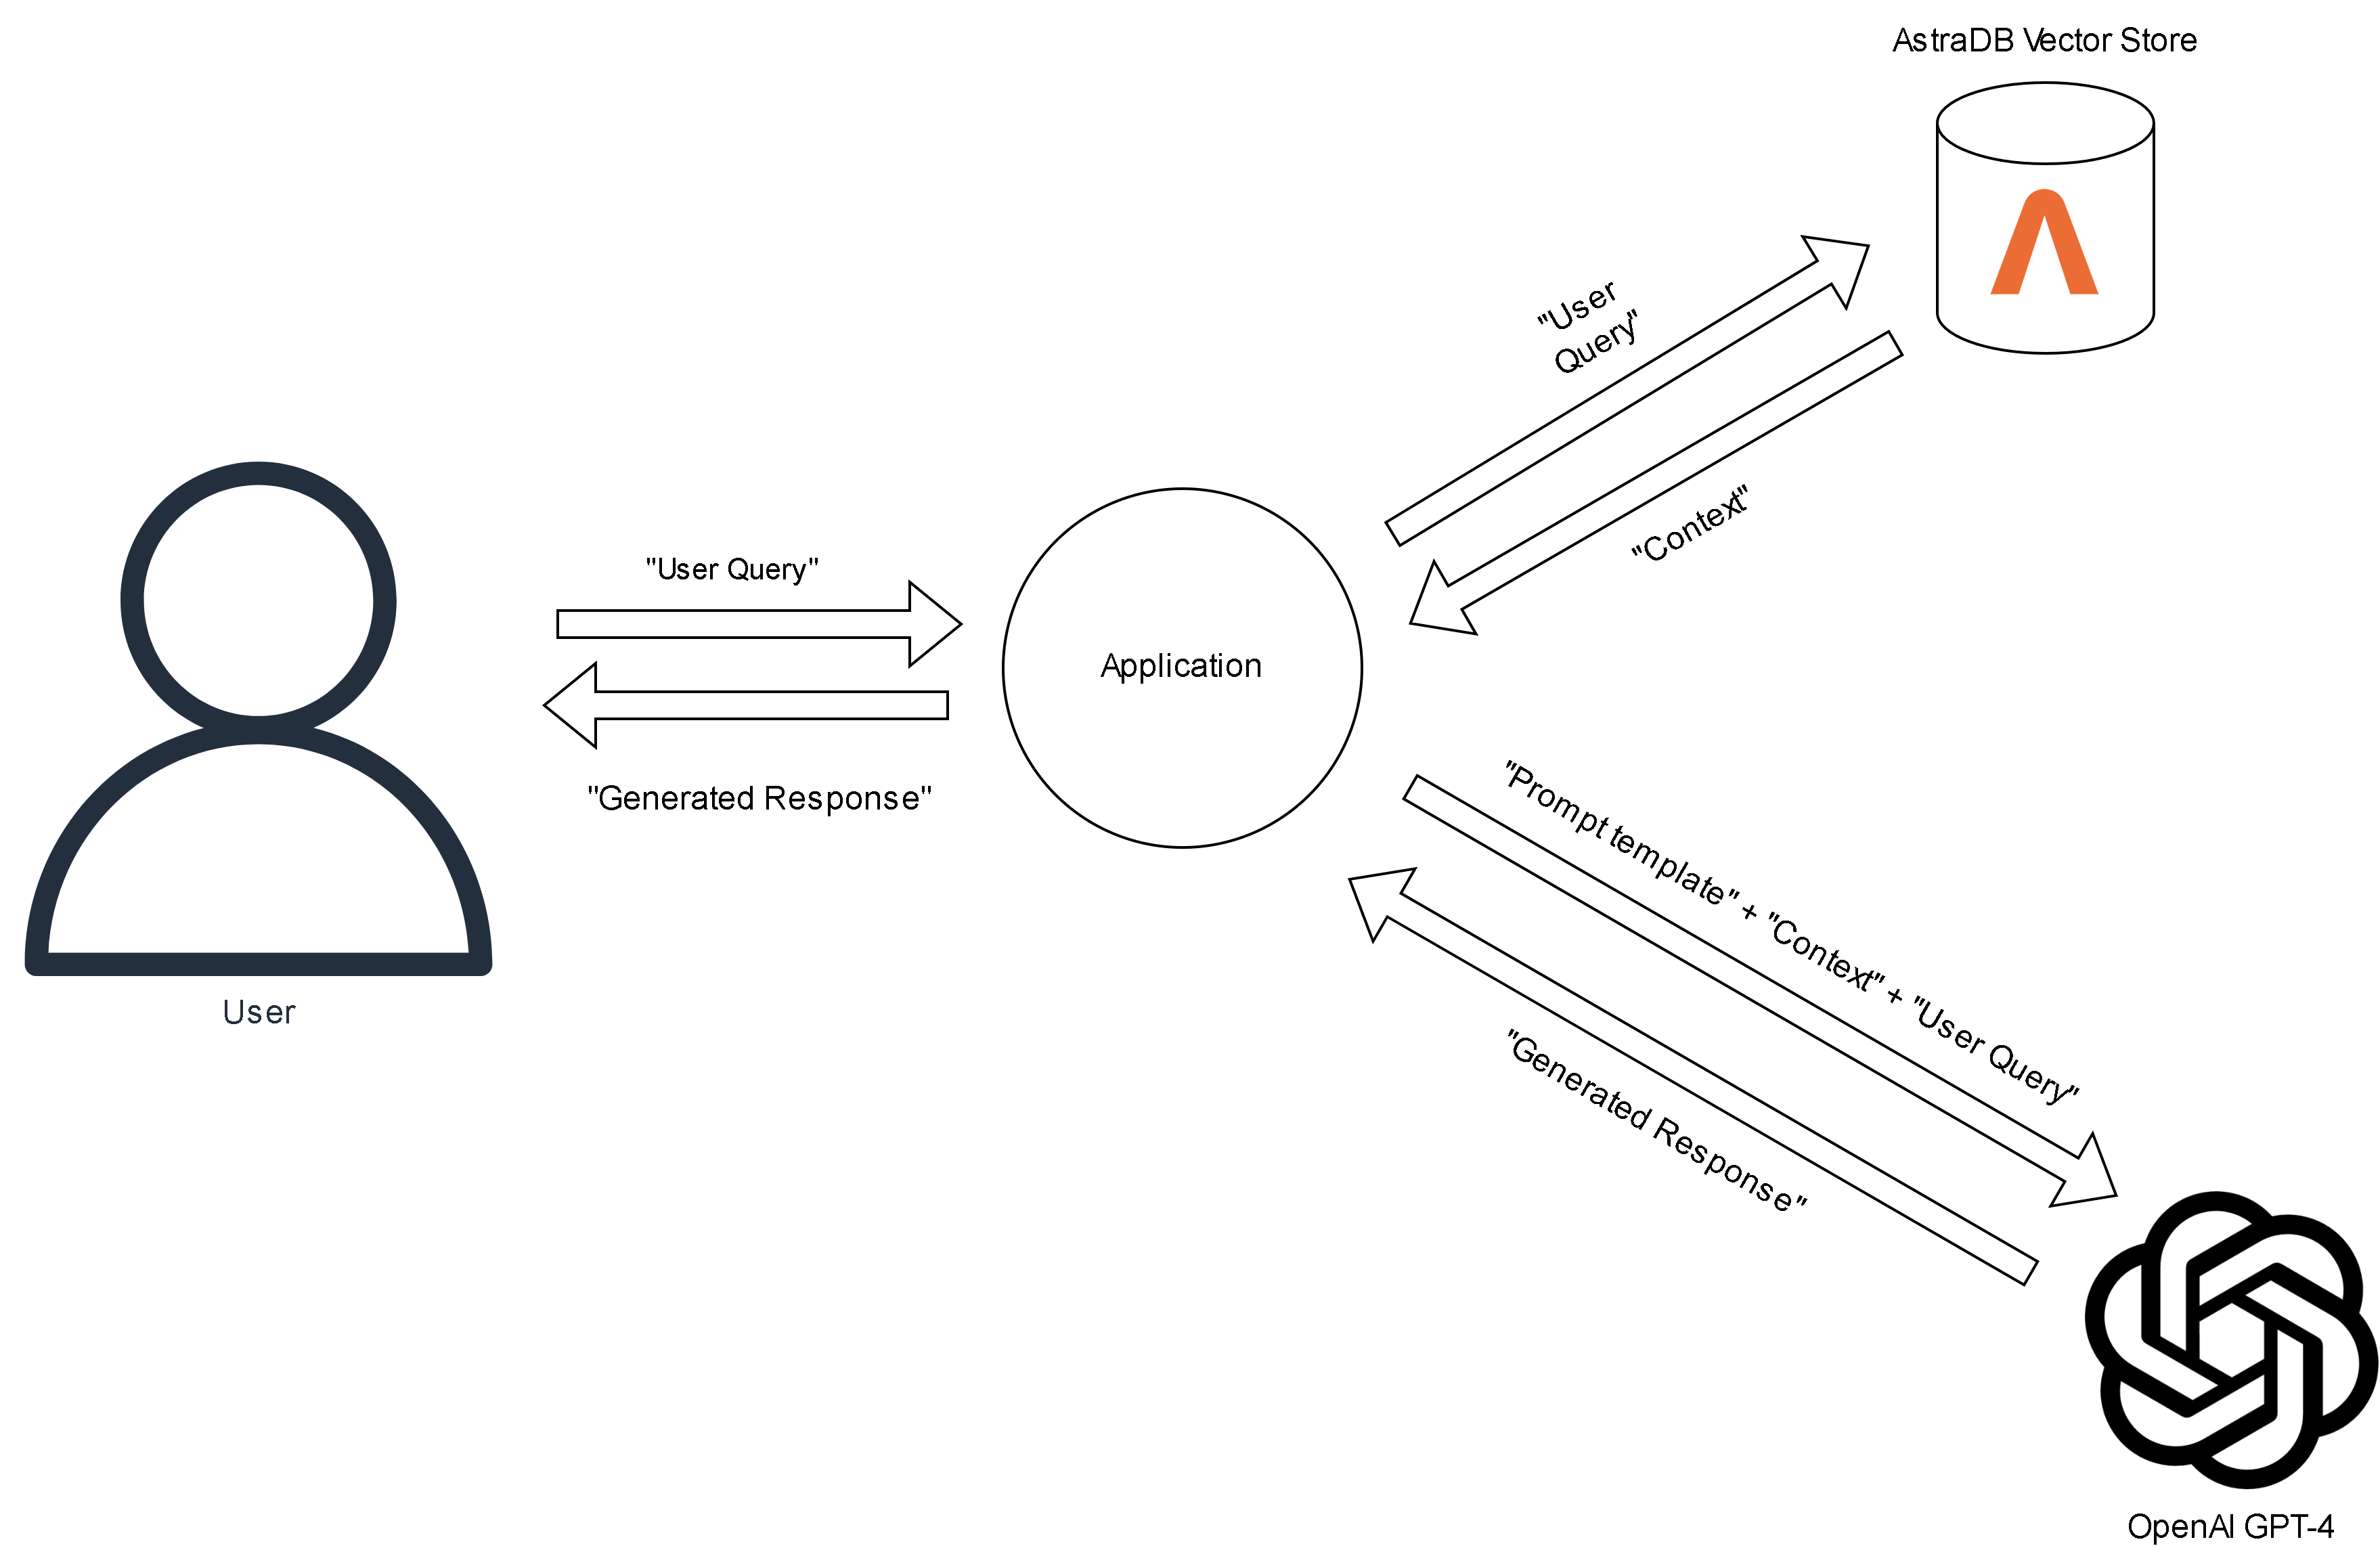
\includegraphics[width=0.8\textwidth]{figs/Chatbot_process.png}
        \caption{Diagram of Query Process}
        \label{fig:rag_chatbot}
    \end{figure}


    



\section{LLM Optimization}
    Optimizing Large Language Models (LLMs) for efficiency and performance without compromising their effectiveness is a critical area of research in the field of artificial intelligence. Various techniques have been developed to address this challenge, each employing unique strategies to reduce computational resources, decrease model size, and maintain, if not improve, the model's performance. This section explores the general methodologies applied in the optimization of LLMs, focusing particularly on model compression techniques. Among these, Low-Rank Approximation stands out as a highly effective approach. This technique leverages the mathematical properties of matrices to approximate the original model parameters with fewer components, thereby possibly reducing the model's computations and resource requirements.

    \subsection{Optimization Techniques for Large Language Models}
        Optimization strategies for Large Language Models (LLMs) are crucial for improving computational efficiency and model efficacy. These strategies are generally divided into two primary types: model pruning and parameter sharing.

        \subsubsection{Model Pruning}
        Model pruning aims to reduce the model's complexity and size effectively without substantial loss in performance. It involves systematically eliminating parameters or connections within the model that are least consequential to the output, thereby enhancing operational efficiency and making the model more adaptable for use in environments with limited resources.

        \subsubsection{Parameter Sharing}
        Conversely, parameter sharing utilizes the model's existing parameters across various parts of the model or different tasks. This method optimizes the use of the model's capacity, enabling multifunctional performance without an increase in parameter count.

        \subsubsection{Focus on Low-Rank Approximation}
        This thesis will specifically focus on model pruning techniques, with a particular emphasis on low-rank approximation. This approach approximates large matrices or tensors with ones of a lower rank, reducing the number of components and computational demands while preserving the model's critical information processing capabilities.


\section{Case Study: Low-Rank Approximation}
    To assess the effectiveness of low-rank approximation in compressing LLMs, we consider Facebook's the BART-Base model (\cite{lewis2019bart}) as a case study. BART is a transformer-based LLM that has been widely used for various natural language processing tasks such as summarization.%\ref{sec:bart}

    This thesis focuses on applying low-rank approximation specifically to the attention matrices. This choice stems from their pivotal role in the transformer architecture. These matrices, which help the model assess the relevance of different words within the input data, tend to be large and often encapsulate redundant information (\cite{aghajanyan2020intrinsic}). %By reducing the dimensionality of these matrices, we preserve the model's ability to perform complex relational reasoning with less computational overhead, thus maintaining efficacy in summarization tasks while enhancing efficiency.

    By applying low-rank approximation to the attention weight matrices of the BART-base model, we aim to explore the possibility in reducing computational complexity and storage requirements while preserving its performance on a summarization task.
    \subsection{Implementation Steps}
        The implementation of low-rank approximation for BART involves the following steps:
        
        \begin{enumerate}
            \item \textbf{Singular Value Decomposition (SVD):} The attention weight matrices (Key, Query, Value, and Output) of the model are decomposed using SVD to obtain the low-rank approximation.
            \[
            \begin{array}{c}
                Q \\[0.2cm] % adds 0.5 cm space after this row
                V \\[0.2cm] % adds 0.5 cm space after this row
                K \\[0.2cm]
                O
            \end{array}
            \xrightarrow[\text{SVD}]{\hspace*{1cm}}
            \begin{array}{c}
                U_q \ \Sigma_q \ V_q^T \\[0.2cm] % adds 0.5 cm space after this row
                U_v \ \Sigma_v \ V_v^T \\[0.2cm] % adds 0.5 cm space after this row
                U_k \ \Sigma_k \ V_k^T \\[0.2cm]
                U_o \ \Sigma_o \ V_o^T

            \end{array}
            \]

            \item \textbf{Custom Layer Implementation:} A custom layer is implemented to replace the original attention layers with the low-rank approximation.
            \begin{figure}[H]
                \centering
                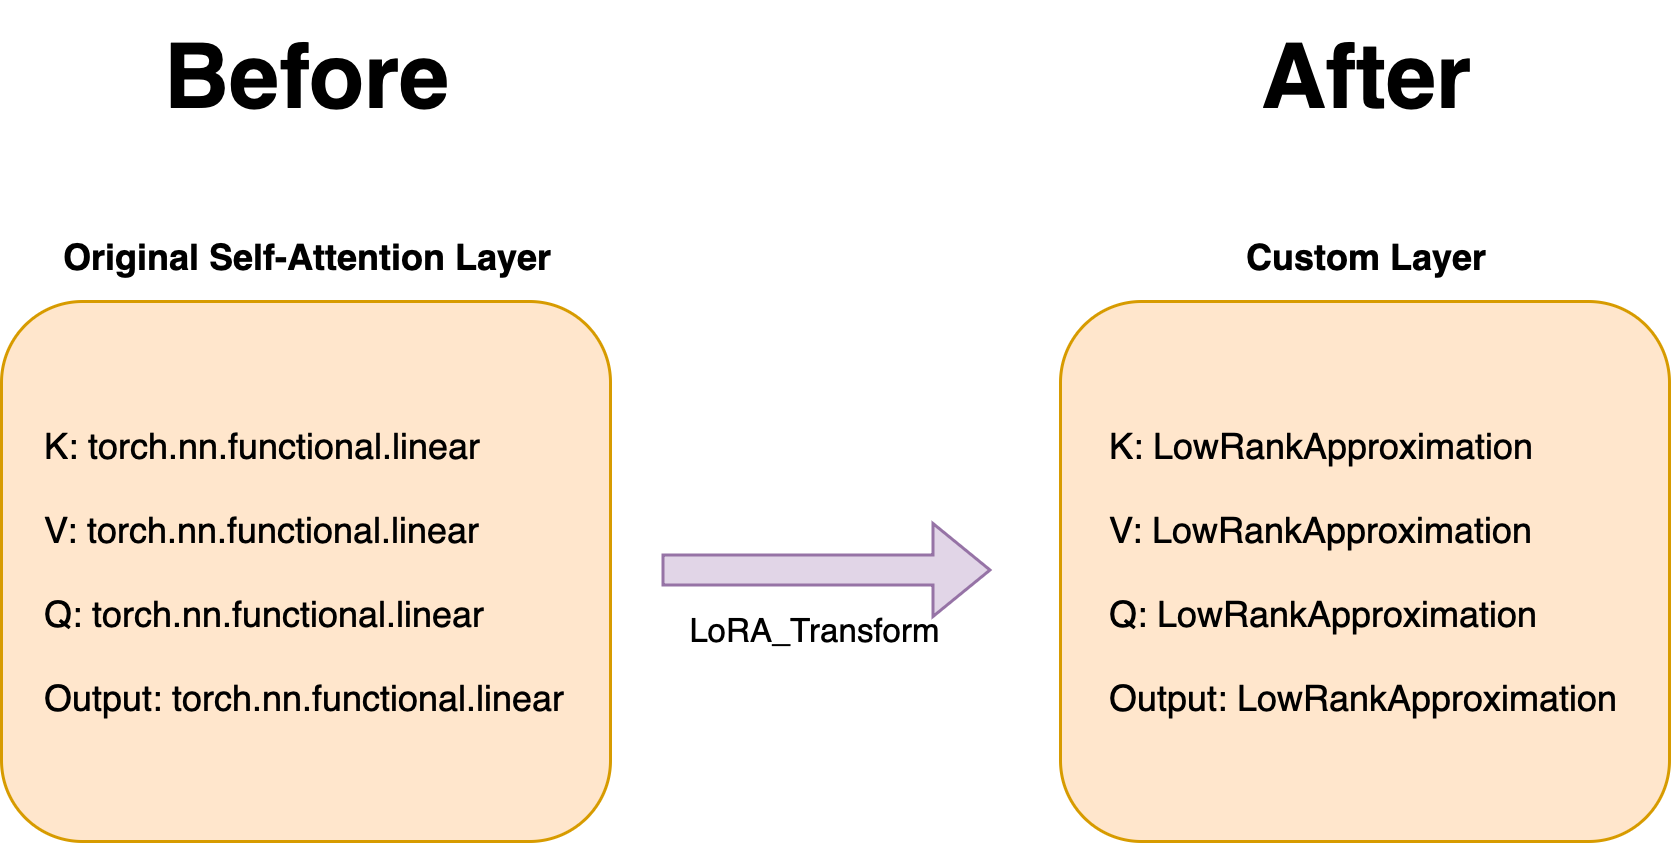
\includegraphics[width=0.7\textwidth]{figs/before-after.png}
                \caption{Components in attention layers replaced with their custom low-rank approximation}
                \label{fig:lora_implementation}
            \end{figure}
        \end{enumerate}
        
        
        
    \subsection{Evaluation Metrics}\label{sec:evaluation_metrics}
        The approximated model is evaluated based on:
        \begin{enumerate}
        \item ROUGE scores (\cite{lin-2004-rouge}): How well does the approximated model perform in comparison to the original BART-Base model on the summarization task? From which rank does the model start to lose performance?
        \item Computational efficiency: How does the approximated model compare to the original BART-Base model in terms of computational resources required?
        \item Cosine similarity: How well does the approximated model maintain the semantic properties of the original model?
        \item Comparing some of the summaries generated by the compressed model with the original BART-Base model and the reference summaries using the Samsum dataset (\cite{gliwa-etal-2019-samsum}).
        \begin{figure}[H]
            \centering
            \includegraphics[width=0.6\textwidth]{figs/dialogue.png}
            \caption{SamSum Dataset \texttt{test[0]} dialogue and reference summary}
            \label{fig:SamSum_Example}
        \end{figure}
        \end{enumerate}

        \subsection{Appropriate Rank Selection}
            In Section \ref{sec:reduction_storage}, we established the criterion for selecting an appropriate rank \(k\) to achieve computational efficiency and storage reduction. The criterion is given by:
            
            \[
            k < \frac{\sqrt{4mn + (m+n)^2} - m - n}{2}
            \]
            
            where \(m\) and \(n\) are the dimensions of the original matrix we wish to approximate with a low-rank representation.
            
            \textbf{BART-base Model:}\\
            For the BART-base model, the attention matrices have dimensions \(m = n = 768\). We know this by inspecting the model's architecture (Appendix \ref{appendix:BART}).\\
            Therefore, the rank \(k\) for the approximation should satisfy:
            \[
            k < \frac{\sqrt{4 \times 768 \times 768 + (768 + 768)^2} - 768 - 768}{2} \approx 318
            \]
            
            \label{appropriate_rank}to achieve a reduction in computational complexity and storage requirements.

            \textbf{BART-large Model:}\\
            Similarly, for the BART-large model, the attention matrices have dimensions \(m = n = 1024\). Therefore, the rank \(k\) for the approximation should satisfy:
            \[
            k < \frac{\sqrt{4 \times 1024 \times 1024 + (1024 + 1024)^2} - 1024 - 1024}{2} \approx 424
            \]
            To determine the feasibility of low-rank approximation for the two BART models, we will evaluate the approximated model at various ranks and observe the impact on the ROUGE scores and the other metrics mentioned in section \ref{sec:evaluation_metrics}. This evaluation will help us understand the trade-offs between rank reduction and model performance.
            

            

        %\textbf{Rank Selection:} The rank of the approximation is chosen based on the observed spectrum decay of the ROUGE-scores, ensuring a balance between speed and task performance retention.

